% This is samplepaper.tex, a sample chapter demonstrating the
% LLNCS macro package for Springer Computer Science proceedings;
% Version 2.20 of 2017/10/04
%
\documentclass[runningheads]{llncs}
% 
\usepackage{graphicx}
\usepackage{listings}
% Used for displaying a sample figure. If possible, figure files should
% be included in EPS format.
%
% If you use the hyperref package, please uncomment the following line
% to display URLs in blue roman font according to Springer's eBook style:
% \renewcommand\UrlFont{\color{blue}\rmfamily}
\usepackage{lettrine} % Pacote para formatação especial da primeira letra
\usepackage{hyperref}

% Define custom settings for listings
\lstset{
    breaklines=true,
    breakatwhitespace=true,
    basicstyle=\small\ttfamily,
    numbers=left,
    numberstyle=\tiny,
    frame=tb,
    columns=fullflexible,
    keepspaces=true
}


\begin{document}
%
\title{Big Data Analysis - Technical report}
% Coloca o DOI aqui se o artigo já tiver sido publicado; caso contrário, deixa como "To be assigned"
% If the paper title is too long for the running head, you can set
% an abbreviated paper title here
%
\author{Diogo Esteves \and Rui Sousa}
%
\authorrunning{Esteves, D. and Sousa, R.}
% First names are abbreviated in the running head.
% If there are more than two authors, 'et al.' is used.
%
\institute{Department of Informatics, University of Minho, Portugal\\
\email{pg28935@alunos.uminho.pt\inst{1} pg21019@alunos.uminho.pt}\inst{2}\\
\url{http://www.di.uminho.pt}}

\maketitle \begin{abstract}
This document aims to provide a detailed explanation of the technical steps assumed to achieve the results and materials discussed on the article "Correlating Obesity and Mental Illnesses".
\end{abstract}
%
%
%
\section{Introduction}

To conduct thorough data analysis, we utilized the Pandas Python package for data manipulation and stored the merged dataset in MongoDB. The data was pre-treated and analyzed using a suite of Python data analytics tools, including Pandas, and visualized using Microsoft Power BI.

We chose MongoDB for its flexible schema design and scalability, which facilitates the storage of diverse data types and accommodates evolving data needs \cite{mongodbarchguide}. MongoDB's document-based model allows for easy integration and retrieval of complex data structures, making it an ideal choice for our analysis, which requires handling various datasets with different formats.

Pandas was selected due to its robust data manipulation capabilities. With Pandas, we can effortlessly clean, transform, and analyze the MongoDB collections, thanks to its intuitive syntax and versatile data structures \cite{pandasdocs}. The DataFrame object in Pandas is particularly powerful, enabling efficient data processing and analysis. Additionally, Pandas integrates well with MongoDB, allowing for seamless data import and export between the two platforms.

The initial step involved importing data from MongoDB into Pandas DataFrames. This allowed us to leverage Pandas' extensive functionality for data cleaning, such as handling missing values, removing duplicates, and standardizing data formats. We also performed exploratory data analysis (EDA) to understand the underlying patterns and distributions within the data. This included generating summary statistics, visualizing data distributions, and identifying potential outliers.

For the visualization aspect, we employed Microsoft Power BI, which provides advanced visualization tools and interactive dashboards. Power BI's integration with Python allowed us to use scripts for more complex visualizations and data transformations, enhancing our ability to present the data insights effectively.

The entire data analysis process was iterative, involving continuous refinement of data cleaning and transformation steps based on the findings from EDA. This iterative approach ensured that the data was in optimal condition for the final analysis and visualization stages. By combining the strengths of MongoDB, Pandas, and Power BI, we were able to create a comprehensive and flexible data analysis pipeline, capable of handling the complexities of our multi-faceted datasets.

\subsection{Data sourcing}

The datasets utilized in this research project are sourced from the \href{https://ourworldindata.org/}{Our World in Data repository}. We have selected distinct datasets that examine the incidence and prevalence of mental diseases, obesity, education levels, and poverty over time.

The obesity dataset examines a wide range of characteristics associated with obesity and its correlations, including mortality rates, risk of coronary diseases, and gender-specific prevalence. For the purposes of this study, we will focus on the percentage of adults who are overweight or obese and the overall prevalence of obesity in adults \cite{Obesity}.

The dataset on mental illnesses, like the previously mentioned datasets, examines the prevalence, burden of disease, and risk factors of various mental illnesses worldwide. Our focus will be exclusively on the prevalence of mental disorders, specifically depression, bipolar disorder, anxiety disorder, and schizophrenia. Additionally, we will attempt to link the eating disorder data within this dataset to the obesity statistics\cite{MentalHealth}.

\subsection{Data Pre-processing with Python Pandas}

Prior to conducting data analysis, we implemented a straightforward data pre-processing pipeline using Python Pandas. This pipeline involved several key steps to ensure the data sets were ready for analysis.

Firstly, we performed data cleaning procedures to address any inconsistencies or errors within the datasets. This included handling missing values, standardizing data formats, and addressing any outliers or anomalies present in the data.

Next, we trimmed the datasets to ensure they all had the same time frame, facilitating easier comparison and analysis across different datasets. This step involved selecting a common time period or range and filtering the data accordingly.

Additionally, we removed any duplicate entries from the datasets to eliminate redundancy and ensure data integrity. Duplicate entries can skew analysis results and lead to inaccurate conclusions, so it was crucial to identify and remove them before proceeding with analysis.

Furthermore, we standardized all columns across the datasets to ensure uniformity and consistency in data representation. This involved aligning column names, data types, and formats to facilitate seamless integration and analysis.

Finally, we merged the pre-processed datasets into a single, comprehensive dataset, which was then saved as a CSV file for ease of exporting to MongoDB or other storage platforms.

The script used to perform these data pre-processing steps is provided below for reference:

\begin{lstlisting}[language=Python,caption={Handling data with Python Pandas},label={lst:example}]

import pandas as pd

# Dataset on world population
pop = pd.read_csv('../datasets/raw/population.csv')
pop.rename(columns={'Entity': 'Country'}, inplace = True)
pop = pop[pop['Year'] >= 1990]
pop = pop[pop['Year'] <= 2016]
pop.head()

# Dataset on obesity
obes = pd.read_csv('../datasets/raw/share-of-adults-defined-as-obese.csv')
obes.rename(columns={'Entity': 'Country'}, inplace = True)
obes = obes[obes['Year'] >= 1990]
obes = obes[obes['Year'] <= 2016] 
obes.head()

# Dataset on mental disorders prevalence
mental = pd.read_csv('../datasets/raw/mental-illnesses-prevalence.csv')
mental.rename(columns={'Entity': 'Country'}, inplace = True)
mental = mental[mental['Year'] >= 1990]
mental = mental[mental['Year'] <= 2016] 
mental.head()

# Merging the dataframes
dataframes = [pop, obes, mental]

fused = dataframes[0]

for dataframe in dataframes[1:]:
    try:
        fused = pd.merge(
            fused,
            dataframe,
            on = ['Country', 'Year', 'Code'],
            how = 'inner'
        )
    except KeyError:
        fused = pd.merge(
            fused,
            dataframe,
            on = ['Country', 'Year'],
            how = 'outer'
        )

# Exporting to CSV
fused.to_csv('../datasets/processed/pd_processed_data.csv')
\end{lstlisting}

\subsection{Exploring Alternative Pre-processing with Spark}

To experiment with different technologies and processing methods, we utilized Apache Spark, leveraging the PySpark library. While our findings yielded similar results to those obtained using other tools, we observed notable differences in processing time between Spark and Pandas.

For instance, Pandas completed the pre-processing task in approximately 0.1 seconds, whereas Spark took around 0.5 seconds to accomplish the same task. This difference, albeit negligible, underscores that for smaller datasets Pandas can be a powerful option. However, Spark's strength lies in its ability to handle larger-scale datasets efficiently.

Therefore, while Spark may not be the optimal choice for every pre-processing task, particularly for smaller datasets, its capabilities shine when dealing with large-scale data operations. The selection of pre-processing tools should be tailored to the specific requirements and characteristics of the dataset, ensuring optimal performance and efficiency.

Below we share the Python script used to handle data with PySpark:

\begin{lstlisting}[language=Python,caption={Handling data with Python PySpark},label={lst:example}]

# Import required libraries
from pyspark.sql import SparkSession
from pyspark.sql.functions import col

# Initialize SparkSession
spark = SparkSession.builder \
    .appName("Pandas to PySpark") \
    .getOrCreate()

# Load datasets
pop = spark.read.csv('../datasets/raw/population.csv', header=True)
obes = spark.read.csv('../datasets/raw/share-of-adults-defined-as-obese.csv', header=True)
mental = spark.read.csv('../datasets/raw/mental-illnesses-prevalence.csv', header=True)

# Rename columns
pop = pop.withColumnRenamed('Entity', 'Country')
obes = obes.withColumnRenamed('Entity', 'Country')
mental = mental.withColumnRenamed('Entity', 'Country')

# Merge datasets
fused = pop.join(obes, ['Country', 'Year', 'Code'], 'inner') \
           .join(mental, ['Country', 'Year', 'Code'], 'inner')

# Drop rows with null values
fused = fused.dropna()

# Export to CSV
fused.coalesce(1).write.mode("overwrite").option("header", "true").csv('../datasets/processed/spark_processed_data')

# Stop SparkSession
spark.stop()
\end{lstlisting}

\subsection{Connecting and adding data to MongoDB}

After cleaning the data we have added it to our MongoDB database. To streamline the process we have also resorted to MongoDB's Python connector through the PyMongo library given its simplicity. Below we demonstrate the python script and workflow to achieve the connection.

\subsection{Connecting and adding data to MongoDB}

\begin{lstlisting}[language=Python,caption={Pymongo workflow},label={lst:example}]

from pymongo.mongo_client import MongoClient
from pymongo.server_api import ServerApi

uri = 'YOUR URL'

# Create a new client and connect to the server
client = MongoClient(uri, server_api=ServerApi('YOUR API')) # replace YOUR API with your MongoDB API

# Send a ping to confirm a successful connection
try:
    client.admin.command('ping')
    print("Pinged your deployment. You successfully connected to MongoDB!")
except Exception as e:
    print(e)

# Access database
db = client.get_database("BigData")

# Access/create collection
collection = db.get_collection("ObesPovMen")
collection

# Read CSV file using pandas
csv_file = "../datasets/processed/pd_processed_data.csv"
data = pd.read_csv(csv_file)

# Convert DataFrame to dictionary
data_dict = data.to_dict(orient='records')

# Insert data into MongoDB collection
collection.insert_many(data_dict)

# Close connection
client.close()
\end{lstlisting}

\subsection{Visualizing and Analyzing Data with Power BI}

To present and harness the processed data, we leveraged Microsoft Power BI. Utilizing the \href{https://www.mongodb.com/docs/atlas/data-federation/query/sql/powerbi/connect/}{Power BI MongoDB connector}, we seamlessly ingested data directly from our database. Subsequently, we employed Power BI to craft dashboards, views, and correlations across various datasets, notably examining the relationship between obesity and mental disorders by order of severity.

Employing a diverse array of visuals and tools, we curated interactive and informative dashboards. These visualizations not only facilitated the exploration of complex data relationships but also empowered users to derive actionable insights from the data.

By harnessing Power BI's capabilities, we were able to unlock the full potential of our processed data, enabling stakeholders to gain deeper understanding and make data-driven decisions with confidence. The dashboards can be viewed and interacted by accessing the \href{https://github.com/rezekiz/big-data-analysis/blob/main/powerbi_files/pbi_project.pbit}{PowerBI project on our GitHub repository}.

Examining the correlation between disorder prevalence and population growth yielded some important discoveries in the analysis of eating disorders and mental health trends throughout time. To conduct this analysis, Power BI preprocessing was carefully used to establish data types, create measurements for each variable, and compute case-to-population ratios. A thorough overview was created by counting the total cases of each disease, which served as the basis for a thorough trend analysis. We share below an assortment of the generated visuals, which are analysed on the article.

\begin{figure}[ht!]
\centering

\begin{tabular}{cc} % Defines a 2-column table
  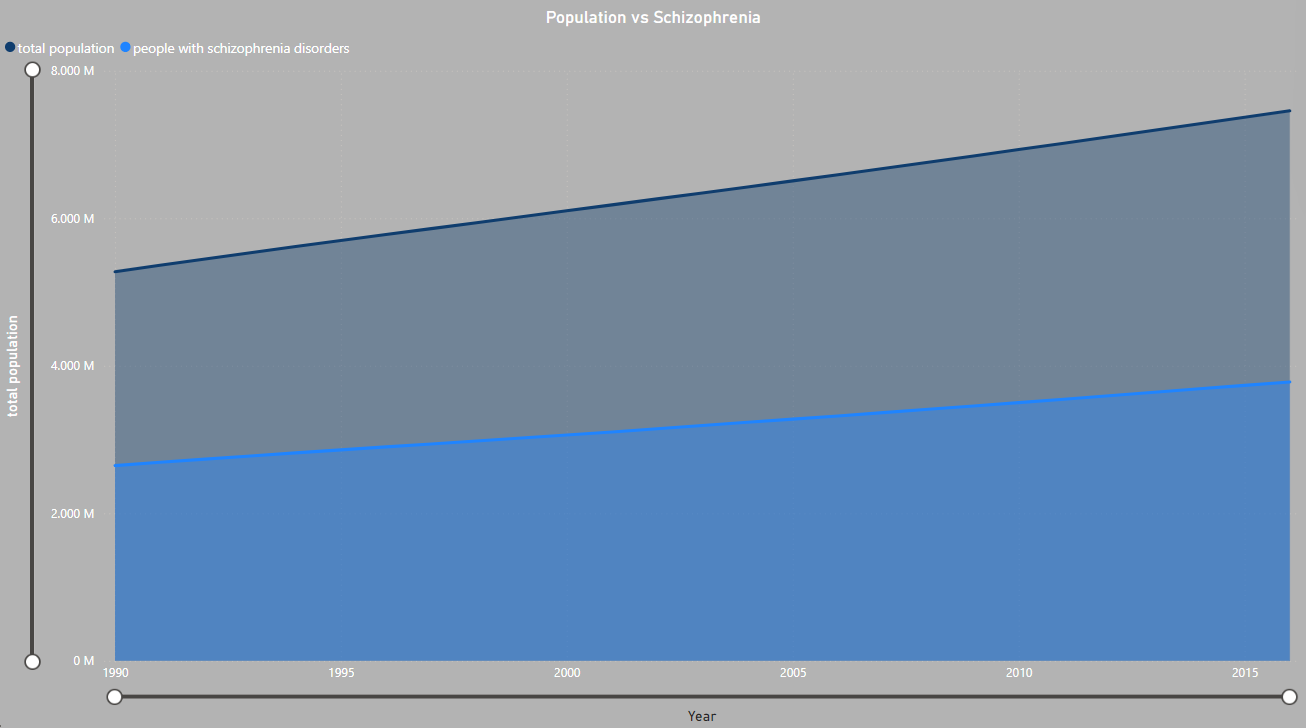
\includegraphics[width=0.5\textwidth]{./imgs/schizo.png} &  % First row, first column
  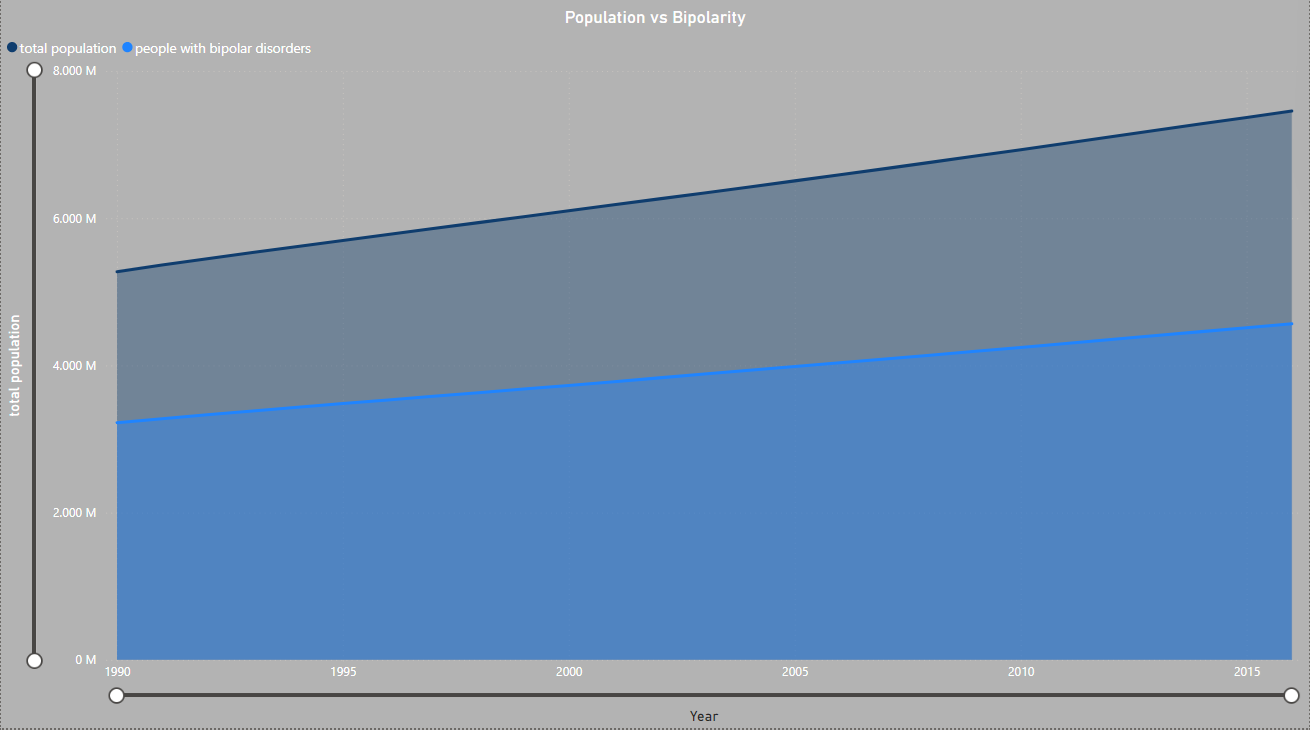
\includegraphics[width=0.5\textwidth]{./imgs/bipolar.png} \\  % First row, second column, line break
  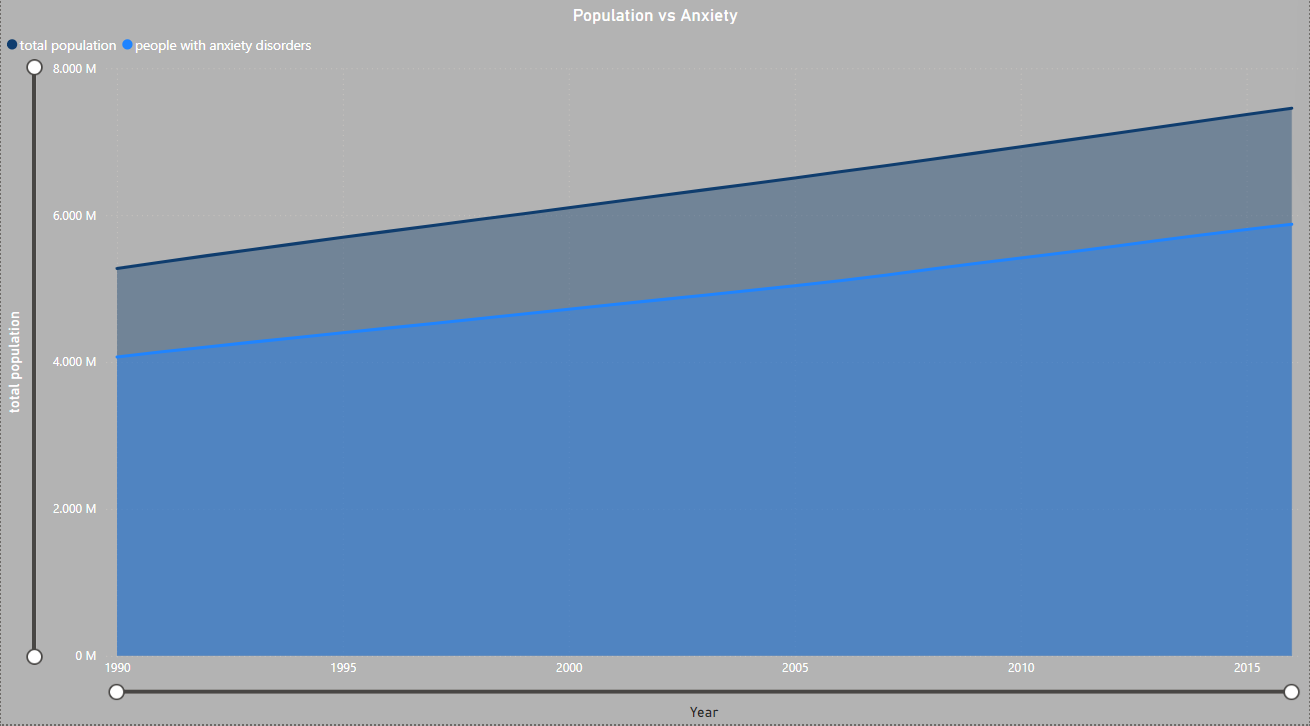
\includegraphics[width=0.5\textwidth]{./imgs/anxiety.png} &  % Second row, first column
  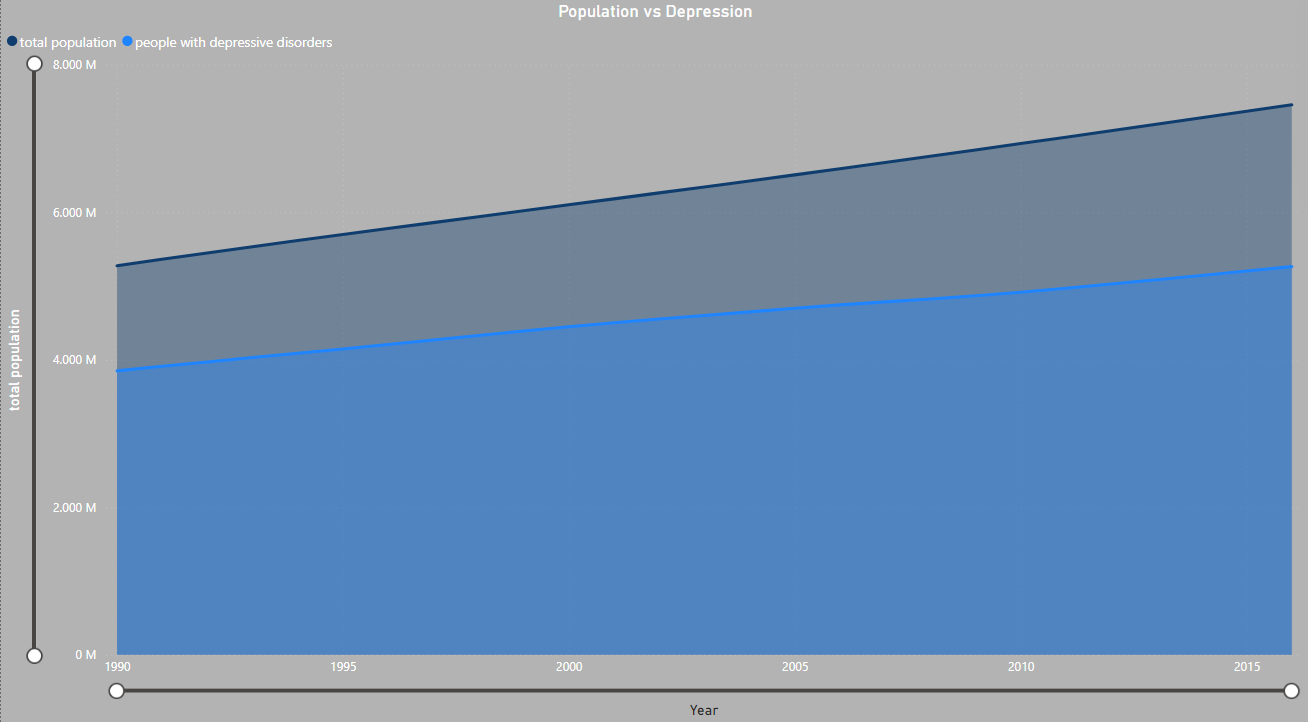
\includegraphics[width=0.5\textwidth]{./imgs/depress.png} \\  % Second row, second column, line break
  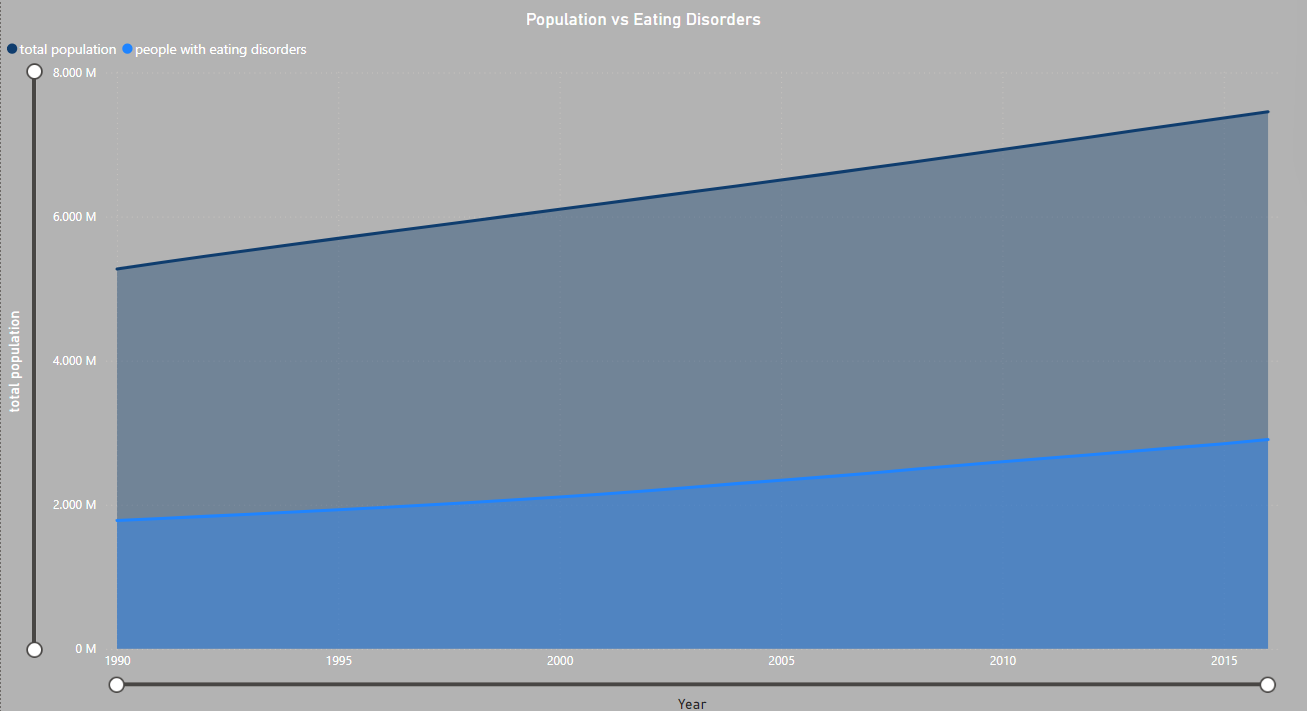
\includegraphics[width=0.5\textwidth]{./imgs/Eating disorders.png} &  % Third row, first column
  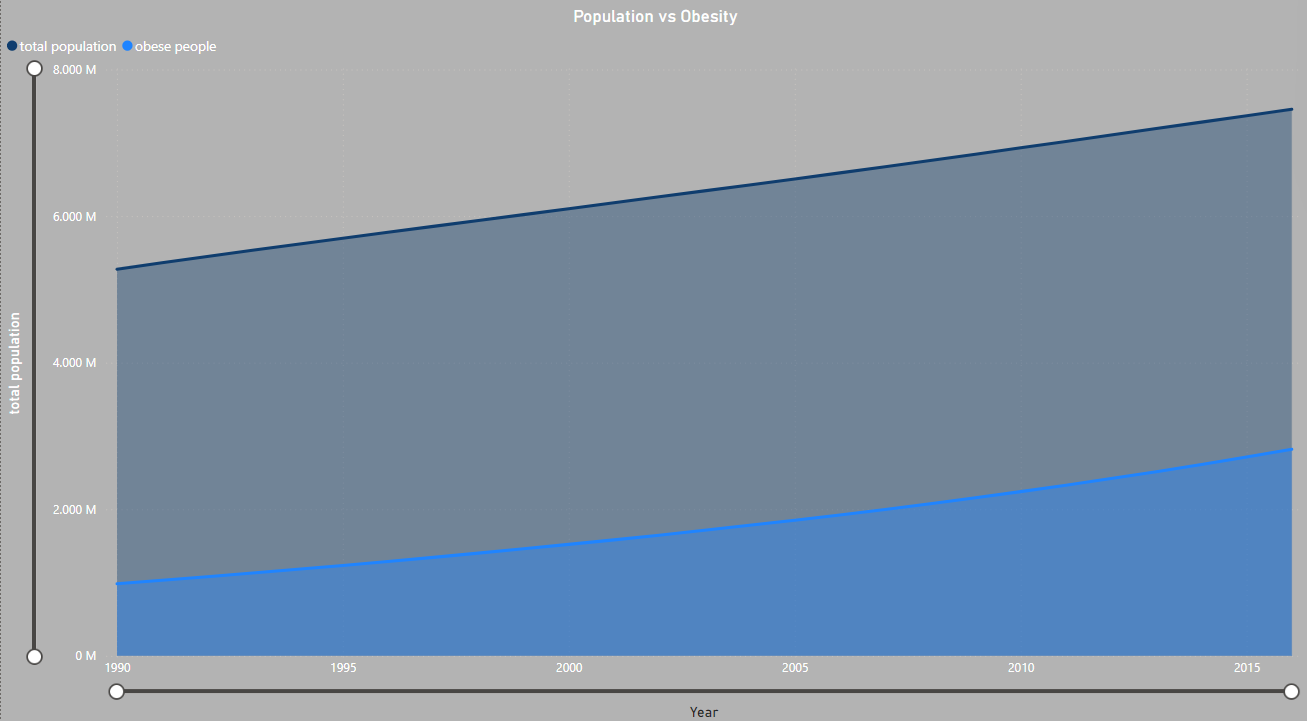
\includegraphics[width=0.5\textwidth]{./imgs/obes.png} \\  % Third row, second column
\end{tabular}

\caption{Mental Health and Population Trends}  % Common caption for all figures
\label{fig:all}
\end{figure}

\clearpage
\section{Final remarks}
This project has advanced our expertise in essential aspects of data management, including cleaning, processing, storage, analysis, and visualization. By employing a range of tools tailored to different stages of the big data pipeline, we have refined our skills and gained practical insights into handling large datasets effectively.

Furthermore, our investigation has uncovered a significant finding in the field of public health: a clear correlation between population growth and the prevalence of eating disorders and mental health issues. This empirical evidence underscores the value of data-driven insights in informing strategic decision-making processes.

By demonstrating the utility of big data analytics in uncovering such critical relationships, our work provides a pragmatic illustration of how data can inform policy formulation and decision-making, ultimately facilitating targeted interventions to address pressing societal challenges, such as the obesity epidemic.

%
% ---- Bibliography ----
%
% BibTeX users should specify bibliography style 'splncs04'.
% References will then be sorted and formatted in the correct style.
%
%\bibliographystyle{splncs04}


\bibliographystyle{unsrt}
\bibliography{bibliography}
%

\end{document}